\section{Overall Reliability}

The final equation of the WRN reliability is a sum of the data and clock distribution reliabilities.
The clock distribution is assumed to be sufficiently accurate as long as there is a connection 
between the TM and all the nodes. The same applies to the CD distribution: 
as long as there is a valid connection, the FEC makes sure that the data is delivered with 
a sufficient reliability and the latency calculations prove it to be deterministic while the 
congestion is prevented by CoS and limited number of data sources (DM). Consequently, the overall 
reliability is strongly dependent on the WRN topology, which needs to be appropriate for the proposed 
solutions (SyncE, H/W-supported RSTP, upper-bound latency). 

For the comparison of different network topologies, we consider the reliability of a network of 
switches. 
%with M inputs (connected to DM/TM). 
Each node is connected to such a network with M links 
(each to a separate switch). The value of M reflects the level of redundancy 
(M=1 for no redundancy, M=2 for double redundancy, etc).


In the calculations of the network reliability we used the idea of Mean Time Between Failure (MTBF) 
and its relation with the failure probability presented in \cite{biblio:mtbf} 
(a very simplified mathematical model). In order to calculate the MTBF of the entire network, we need the 
MTBFs of each network component: switches and links. Since the WR switches are still under 
development (no MTBF measured), we used representative values for CISCO switches 
({2, 10 and 100}$*10^4$[h]). Two estimation methods were used: "Fault Tree analysis" 
\cite{biblio:faultTree} and analytic. Both provide just rough estimations of the reliability. 
The former allowed to estimate two-terminal reliability (DM to single node) 
%\cite{biblio:INF_TECH} 
of simple non/double/triple-redundancy topologies ($P_f$). The most desired value is the 
all-terminal network reliability ($P_{f\_Network}$), where : $P_f < P_{f\_Network} < N_{nodes}*P_f$. 
Table~\ref{tab:2000nodesReliability} 
presents rough estimations of $P_{f\_Network}$ using analytic calculations for the three considered 
topologies ($MTBF_{Switch}$=200 000[h]). However, to meet the requirement of $\approx$2000 nodes and 
only three network layers (hops), 
\modified{the Data Master node is connected to more separate switches than 
the level of redundancy (M).}
% the topologies are of the type M-inputs/N-outputs, where 
% $N \geq M$.
The estimations show that a triple redundancy topology can barely satisfy the requirements by CERN 
(Table~\ref{tab:requirements}).

% \begin{figure}[t]
% 	 \centering
% 	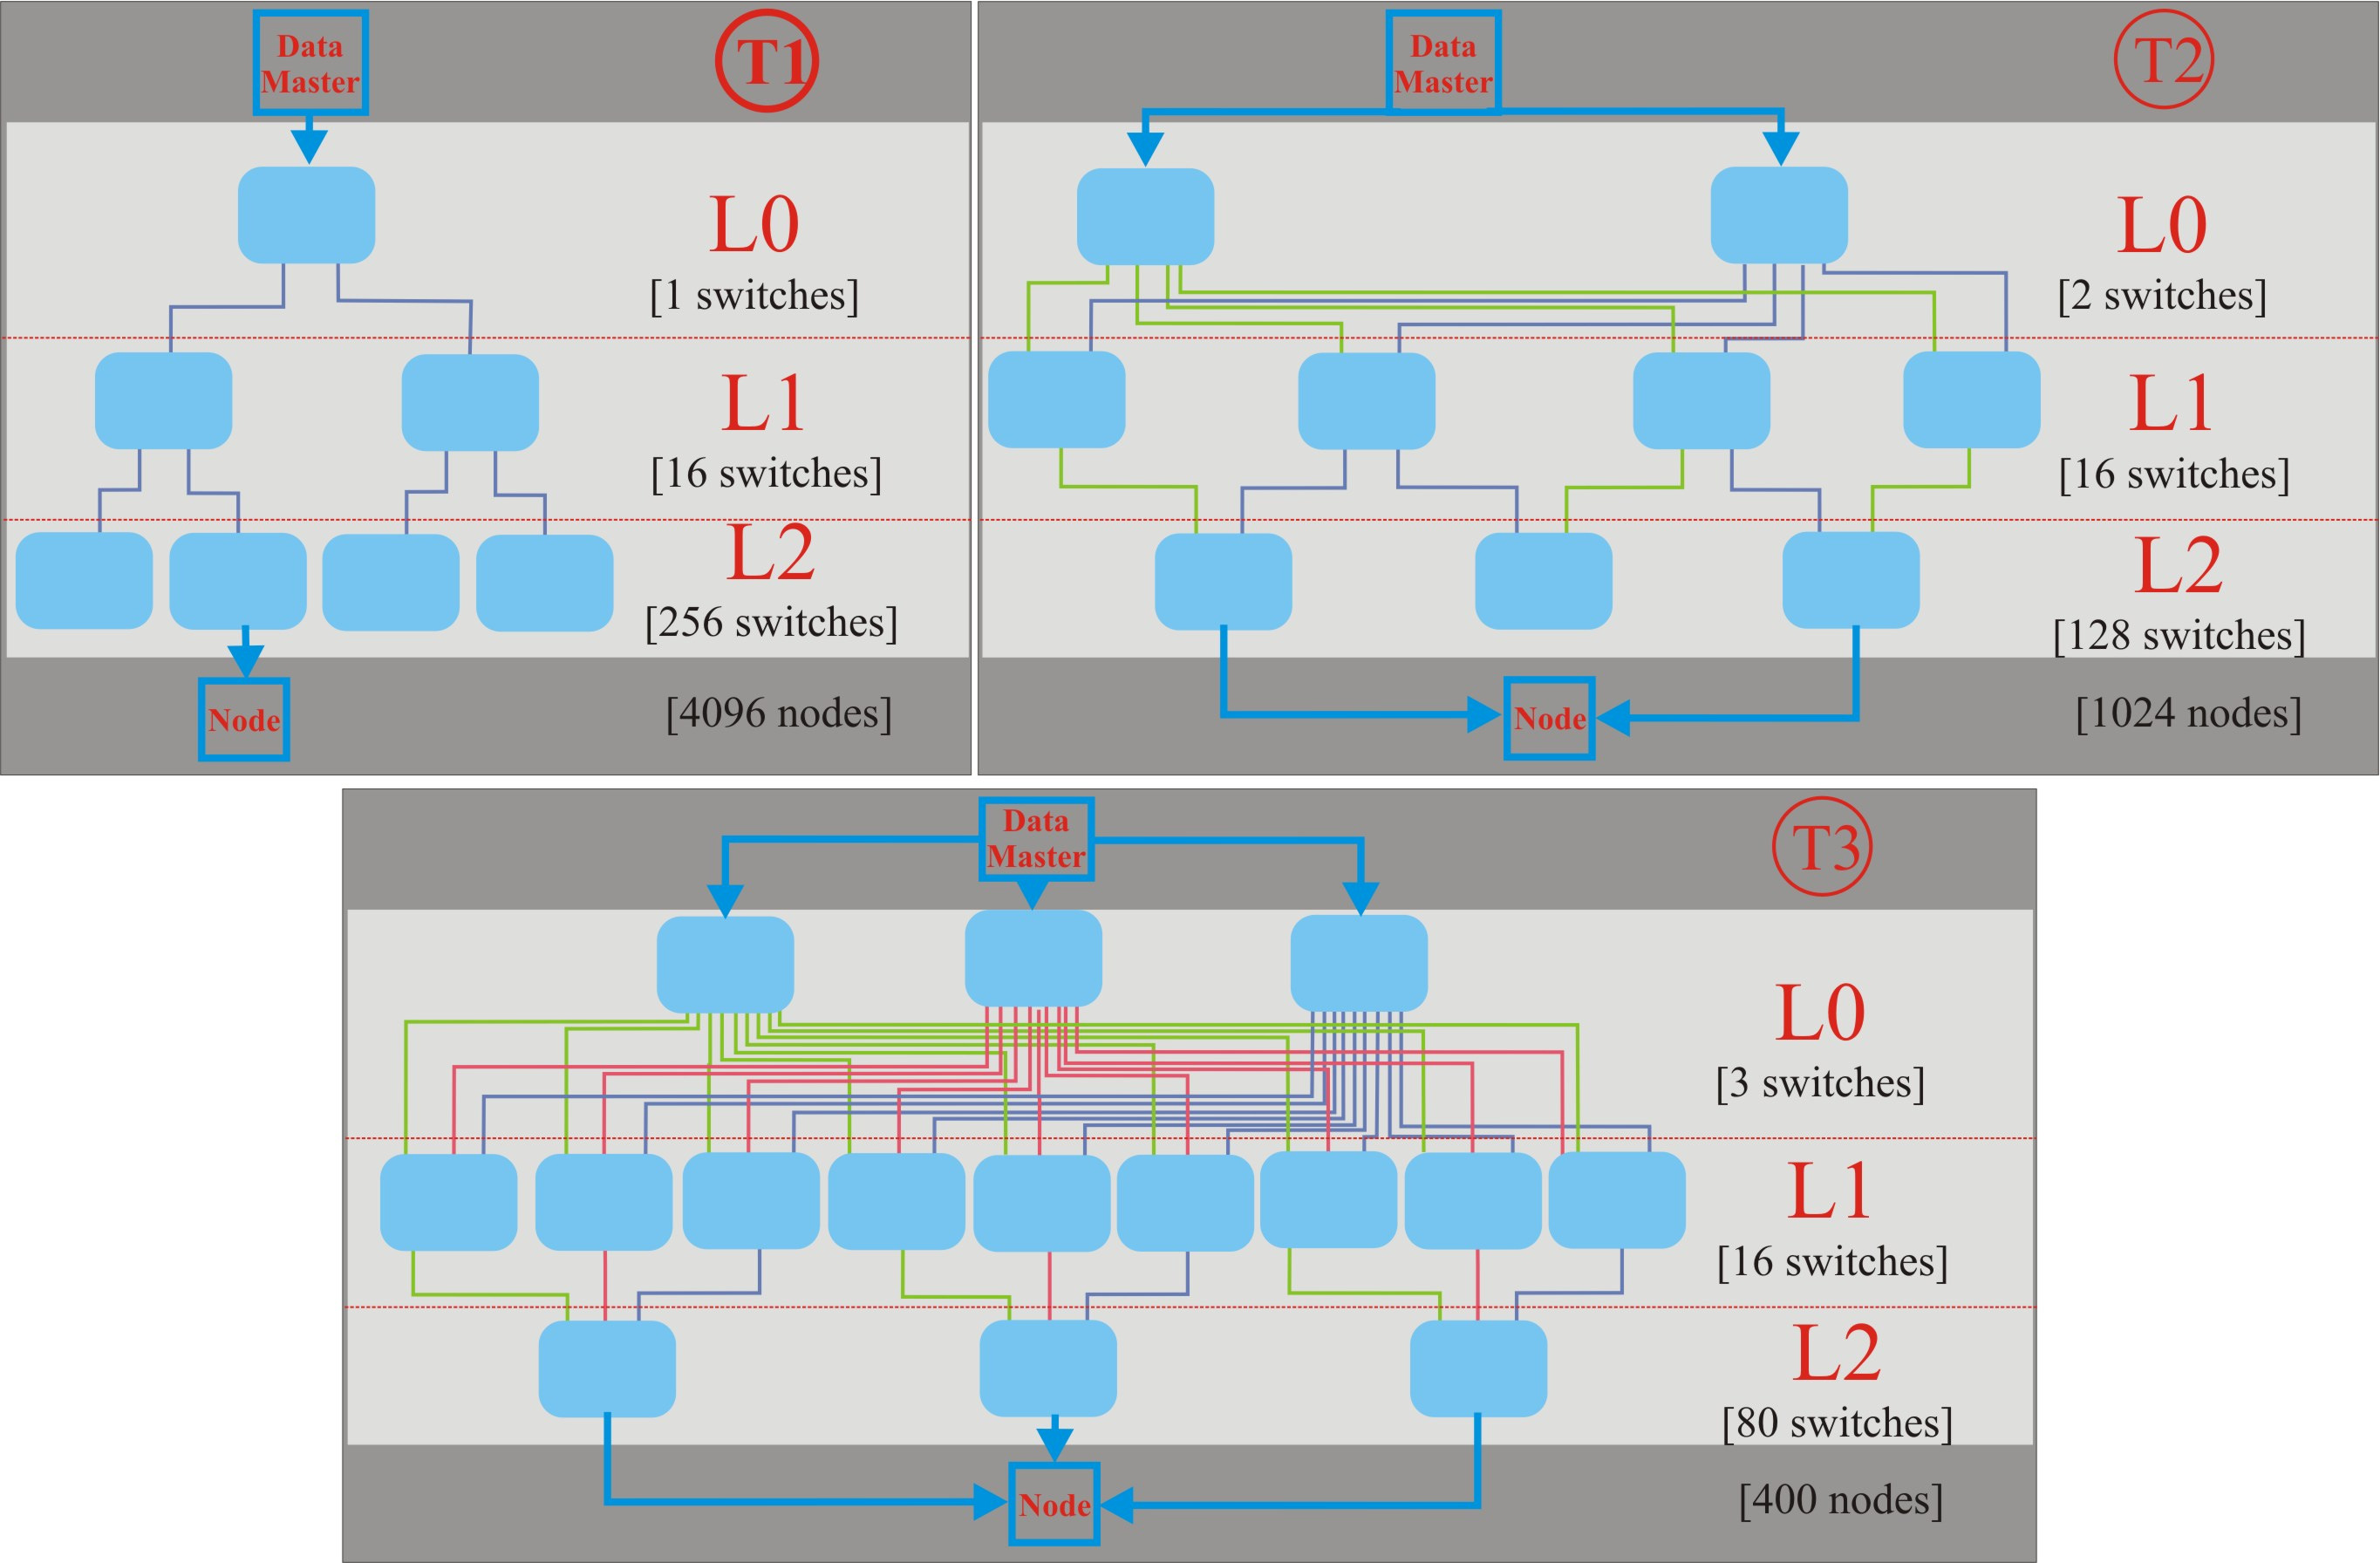
\includegraphics[width=3.4in]{fig/threeTopologies.ps}
% 	\caption{Examples of topologies with different level of redundancy.}
% 	\label{fig:threeTopology}
% \end{figure}

\begin{table}[ht]

%\caption{Different topologies ($\approx 2000$ nodes).}
\caption{WRN topologies's reliabilities.}
\centering
%\rowcolors {0}{gray!35}{}

\begin{tabular}{| c | c | c | c |}        \hline
%{\bf Redundancy}& \textbf{Switches}  & \multicolumn{2}{| c |}{\textbf{$MTBF_{Switch}$=  20 000[h] }} \\
%                &                    & $P_f$                       & MTBF[h]               \\ \hline
\rowcolor{gray!35}{}
{\bf Redundancy}& \textbf{Switches}  & $P_f$                       & MTBF[h]               \\ \hline
No              &  127               & $ 2.08*10^{-3}$             & $ 5.77*10^{3}$        \\ \hline
Double          &  292               & $ 4.71*10^{-7}$             &  $ 2.55*10^{7}$       \\ \hline
Triple          &  495               & $ 3.06*10^{-11}$            &  $ 4.08*10^{11}$      \\ \hline
\end{tabular}
\label{tab:2000nodesReliability}
\end{table}

